\def\year{2020}\relax
%File: formatting-instruction.tex
\documentclass[letterpaper]{article} % DO NOT CHANGE THIS
\usepackage{aaai20}  % DO NOT CHANGE THIS
\usepackage{times}  % DO NOT CHANGE THIS
\usepackage{helvet} % DO NOT CHANGE THIS
\usepackage{courier}  % DO NOT CHANGE THIS
\usepackage[hyphens]{url}  % DO NOT CHANGE THIS
\usepackage{graphicx} % DO NOT CHANGE THIS
\urlstyle{rm} % DO NOT CHANGE THIS
\def\UrlFont{\rm}  % DO NOT CHANGE THIS
\usepackage{graphicx}  % DO NOT CHANGE THIS
\frenchspacing  % DO NOT CHANGE THIS
\setlength{\pdfpagewidth}{8.5in}  % DO NOT CHANGE THIS
\setlength{\pdfpageheight}{11in}  % DO NOT CHANGE THIS

\usepackage{balance}
\usepackage{algorithm}
\usepackage{algorithmic}
\usepackage{graphicx}

\usepackage[colorlinks,linkcolor=black,anchorcolor=black,citecolor=black]{hyperref}

\usepackage{pgf}
\usepackage{tikz}
\usepackage{booktabs}
\usetikzlibrary{arrows, automata, shapes,snakes}
% \usepackage[latin1]{inputenc}
\usepackage[utf8]{inputenc}
\usepackage{array}
\usepackage[labelfont=bf,textfont=bf]{caption}
\captionsetup[figure]{labelfont={bf},name={Figure}}
%\captionsetup[figure]{labelfont={bf},name={Figure},labelsep=period}
%\usepackage[font=normalsize,labelfont=bf]{caption}
%\usepackage[justification=centering]{caption}
\usepackage{color}
%\usepackage{ulem} 
\usepackage{amssymb}

\definecolor{note}{rgb}{0,0,1} %blue
%\definecolor{revise}{rgb}{0,0,0} %black

%\nocopyright
%PDF Info Is REQUIRED.
% For /Author, add all authors within the parentheses, separated by commas. No accents or commands.
% For /Title, add Title in Mixed Case. No accents or commands. Retain the parentheses.
\pdfinfo{
/Title (AutoConfigure: a Content-driven Automatic Configuration Framework for Video Analytics Pipeline)
/Author (Zhaoliang He, Chen Tang, Zhi Wang)
%Zhaoliang He, Chen Tang, Zhi Wang
} %Leave this	
% /Title ()
% Put your actual complete title (no codes, scripts, shortcuts, or LaTeX commands) within the parentheses in mixed case
% Leave the space between \Title and the beginning parenthesis alone
% /Author ()
% Put your actual complete list of authors (no codes, scripts, shortcuts, or LaTeX commands) within the parentheses in mixed case. 
% Each author should be only by a comma. If the name contains accents, remove them. If there are any LaTeX commands, 
% remove them. 

% DISALLOWED PACKAGES
% \usepackage{authblk} -- This package is specifically forbidden
% \usepackage{balance} -- This package is specifically forbidden
% \usepackage{caption} -- This package is specifically forbidden
% \usepackage{color (if used in text)
% \usepackage{CJK} -- This package is specifically forbidden
% \usepackage{float} -- This package is specifically forbidden
% \usepackage{flushend} -- This package is specifically forbidden
% \usepackage{fontenc} -- This package is specifically forbidden
% \usepackage{fullpage} -- This package is specifically forbidden
% \usepackage{geometry} -- This package is specifically forbidden
% \usepackage{grffile} -- This package is specifically forbidden
% \usepackage{hyperref} -- This package is specifically forbidden
% \usepackage{navigator} -- This package is specifically forbidden
% (or any other package that embeds links such as navigator or hyperref)
% \indentfirst} -- This package is specifically forbidden
% \layout} -- This package is specifically forbidden
% \multicol} -- This package is specifically forbidden
% \nameref} -- This package is specifically forbidden
% \natbib} -- This package is specifically forbidden -- use the following workaround:
% \usepackage{savetrees} -- This package is specifically forbidden
% \usepackage{setspace} -- This package is specifically forbidden
% \usepackage{stfloats} -- This package is specifically forbidden
% \usepackage{tabu} -- This package is specifically forbidden
% \usepackage{titlesec} -- This package is specifically forbidden
% \usepackage{tocbibind} -- This package is specifically forbidden
% \usepackage{ulem} -- This package is specifically forbidden
% \usepackage{wrapfig} -- This package is specifically forbidden
% DISALLOWED COMMANDS
% \nocopyright -- Your paper will not be published if you use this command
% \addtolength -- This command may not be used
% \balance -- This command may not be used
% \baselinestretch -- Your paper will not be published if you use this command
% \clearpage -- No page breaks of any kind may be used for the final version of your paper
% \columnsep -- This command may not be used
% \newpage -- No page breaks of any kind may be used for the final version of your paper
% \pagebreak -- No page breaks of any kind may be used for the final version of your paperr
% \pagestyle -- This command may not be used
% \tiny -- This is not an acceptable font size.
% \vspace{- -- No negative value may be used in proximity of a caption, figure, table, section, subsection, subsubsection, or reference
% \vskip{- -- No negative value may be used to alter spacing above or below a caption, figure, table, section, subsection, subsubsection, or reference

\setcounter{secnumdepth}{0} %May be changed to 1 or 2 if section numbers are desired.

% The file aaai20.sty is the style file for AAAI Press 
% proceedings, working notes, and technical reports.
%
\setlength\titlebox{2.5in} % If your paper contains an overfull \vbox too high warning at the beginning of the document, use this
% command to correct it. You may not alter the value below 2.5 in
%\title{AAAI Press Formatting Instructions \\for Authors Using \LaTeX{} --- A Guide }
\title{AutoConfigure: a Content-driven Automatic Configuration Framework for Video Analytics Pipeline}
%Your title must be in mixed case, not sentence case. 
% That means all verbs (including short verbs like be, is, using,and go), 
% nouns, adverbs, adjectives should be capitalized, including both words in hyphenated terms, while
% articles, conjunctions, and prepositions are lower case unless they
% directly follow a colon or long dash
\author{Written by Zhaoliang He\textsuperscript{\rm 1}, \Large \textbf{Chen Tang\textsuperscript{\rm 1}, Zhi Wang\textsuperscript{\rm 2}}\\ % 
\textsuperscript{\rm 1}Department of Computer Science and Techonology, Tsinghua University\\  
\textsuperscript{\rm 2}Tsinghua Shenzhen International Graduate School, Tsinghua University}

%\author{Written by AAAI Press Staff\textsuperscript{\rm 1}\thanks{Primarily Mike Hamilton of the Live Oak Press, LLC, with help from the AAAI Publications Committee}\\ \Large \textbf{AAAI Style Contributions by
%Pater Patel Schneider,} \\ \Large \textbf{Sunil Issar, J. Scott Penberthy, George Ferguson, Hans Guesgen}\\ % All authors must be in the same font size and format. Use \Large and \textbf to achieve this result when breaking a line
%\textsuperscript{\rm 1}Association for the Advancement of Artificial Intelligence\\ %If you have multiple authors and multiple affiliations
%% use superscripts in text and roman font to identify them. For example, Sunil Issar,\textsuperscript{\rm 2} J. Scott Penberthy\textsuperscript{\rm 3} George Ferguson,\textsuperscript{\rm 4} Hans Guesgen\textsuperscript{\rm 5}. Note that the comma should be placed BEFORE the superscript for optimum readability
%2275 East Bayshore Road, Suite 160\\
%Palo Alto, California 94303\\
%publications20@aaai.org % email address must be in roman text type, not monospace or sans serif
%}
\begin{document}
\bibliographystyle{aaai}
\maketitle

\begin{abstract}
The configuration in video analytics defines parameters including frame rate, image resolution, and model selection for video analytics pipeline, and thus determines the inference accuracy and resource consumption. Traditional solutions to select a configuration are either fixed (i.e., the same configuration is used all the time) or periodically adjusted using a brute-force search scheme (i.e., periodically trying different configurations and selecting the one with the best performance), and thus suffer either low inference accuracy or high computation cost to find a proper configuration timely. To this end, we propose a video analytical configuration adaptation framework called AdaConfigure that dynamically selects video configuration without resource-consuming exploration. First, we design a reinforcement learning-based framework in which an agent adaptively chooses the configuration according to the spatial and temporal features of the current video stream. In particular, we use a video segmentation strategy to capture the characteristics of the video stream with much-reduced computation cost: profiling a segment uses only 0.2-2\% computation resource as compared to a full video. Second, we design a reward function that considers both the inference accuracy and computation resource consumption so that the configuration achieves good accuracy and resource consumption tradeoff. Our evaluation experiments on object detection task show that our approach outperforms baseline: it achieves 10-35\% higher accuracy with a similar amount of computation resources or achieves similar accuracy with only 60-90\% of the computation resource.
\end{abstract}

%229 words
%The configuration in video analytics defines parameters including frame rate, image resolution, and model selection for video analytics pipeline, and thus determines the inference accuracy and resource consumption. Traditional solutions to select a configuration are either fixed (i.e., the same configuration is used all the time) or periodically adjusted using a brute-force search scheme (i.e., periodically trying different configurations and selecting the one with the best performance), and thus suffer either low inference accuracy or high computation cost to find a proper configuration timely. To this end, we propose a video analytical configuration adaptation framework called AdaConfigure that dynamically selects video configuration without resource-consuming exploration. First, we design a reinforcement learning-based framework in which an agent adaptively chooses the configuration according to the spatial and temporal features of the current video stream. In particular, we use a video segmentation strategy to capture the characteristics of the video stream with much-reduced computation cost: profiling a segment uses only 0.2-2\% computation resource as compared to a full video. Second, we design a reward function that considers both the inference accuracy and computation resource consumption so that the configuration achieves good accuracy and resource consumption tradeoff. Our evaluation experiments on object detection task show that our approach outperforms baseline: it achieves 10-35\% higher accuracy with a similar amount of computation resources or achieves similar accuracy with only 60-90\% of the computation resource. 

%zhaoliang
%Deep convolutional neural networks (NN)-based video analytics services demand intensive computation resources and high inference accuracy. Static configuration would either waste computation resources (by picking the highest frame rate and resolution) or decrease inference accuracy. Knowing this, adapting video configuration is still extremely challenging: 1) The best video configuration is determined by confounding factors, including the characteristics of the input video, the various accuracy-demand services, and computation resource, etc. 2) The cost of adaptive configuration profiling may far exceed the benefits of adaptive configurations. To tackle these challenges, we propose a reinforcement learning-based video analytics configuration framework, AdaConfigure. In particular, we design an agent that adaptively chooses the configuration according to the spatial and temporal features of video contexts. The design of reward carefully considers accuracy and computation resources to assess the impact of each configuration, guiding the agent learning to choose the best configuration for different accuracy-demand services. We leverage dividing video strategy and the extremely short choosing action time of agent to reduce profiling cost, which is only 0.2-2\% overhead to the overall video analytics services. Our evaluation experiments using the object detection task show that our approach outperforms static configurations by achieves 10-35\% higher accuracy with a similar amount of computation resources or achieves similar accuracy with only 60-90\% of the computation resources.

%We design a reward with comprehensive considering of accuracy and computation resources to assess each configuration's impact,

%2) It is hard to assess the impact that each configuration change will produce. 

%Deep convolutional neural networks (NN)-based video analytics services demand intensive computation resources and high inference accuracy. Due to the highly variable video context, the \emph{best} configuration also varies over time. If one chooses a static configuration (i.e., only profiles the video stream to choose the best configuration \emph{once}), the services would either waste computation resources (by picking an expensive configuration) or decrease inference accuracy. Conversely, searching for all configurations in an enormous space can lead to excessive resource overhead that far exceeds the benefits of periodic configurations. Knowing this, designing an \emph{adaptive} approach to choose the best configuration for the current video context is meaningful. We propose a reinforcement learning (RL)-based adaptive video analytics configuration framework, AutoConfigure. The unique feature of AutoConfigure is \emph{context-driven}, meaning that AutoConfigure can adapt the best configuration to intrusive dynamics of video contexts. In particular, our solution can choose the best configuration for the current video chunk according to the spatial and temporal features of video contexts. We implement and evaluate this approach in the object detection task, comparing its performance to static configuration. We show that AutoConfigure achieves 10-35\% higher accuracy with a similar amount of computation resources or achieves similar accuracy with only 60-90\% of the computation resources. Our solution proves to be more efficient than static solutions and only creates an overhead of 0.1-1\% to the overall video analytics services.
%and dynamic configuration baseline

%\noindent Congratulations on having a paper selected for inclusion in an AAAI Press proceedings or technical report! This document details the requirements necessary to get your accepted paper published using PDF\LaTeX{}. If you are using Microsoft Word, instructions are provided in a different document. AAAI Press does not support any other formatting software. 
%
%\begin{itemize}
%\item You must use the 2020 AAAI Press \LaTeX{} style file and the aaai.bst bibliography style file, which are located in the 2020 AAAI Author Kit (aaai20.sty and aaai.bst).
%\item You must complete, sign, and return by the deadline the AAAI copyright form (unless directed by AAAI Press to use the AAAI Distribution License instead).
%\item You must read and format your paper source and PDF according to the formatting instructions for authors.
%\item You must submit your electronic files and abstract using our electronic submission form \textbf{on time.}
%\item You must pay any required page or formatting charges to AAAI Press so that they are received by the deadline.
%\item You must check your paper before submitting it, ensuring that it compiles without error, and complies with the guidelines found in the AAAI Author Kit.

%\end{itemize}

\section{Introduction}

\label{Section: introduction}
%With the increasing demand for continuous video analytics in public safety and transportation, more and more cameras are being deployed to various locations. The video analytics are based on classical computer vision techniques as well as deep convolutional neural networks. In recent years, we have also witnessed the emergence of a large number of excellent models for target detection \cite{trade-offs}, such as FasterRCNN \cite{ren2015faster_rcnn}, RFCN \cite{dai2016r_fcn}, Multibox \cite{szegedy2014multibox}, SSD \cite{liu2016ssd} and YOLO \cite{redmon2016yolo}.
%For the collected video, the classical computer vision and deep neural network technology are generally used for video analytics. 
A video analytics application consists of a \emph{pipeline} of several video processing modules, typically including a decoder, a selective sampling frame application, and a target detector. Such a pipeline always has multiple \emph{knobs}, such as frame rate, resolution,  detector model selection and so on. A combination of the knob values is video analytics \emph{configuration}, and the configuration space grows \emph{exponentially} with the number of knobs and their values \cite{jiang2018chameleon}.
%(e.g., SSD \cite{liu2016ssd}+{MobileNet \cite{MobileNetV2}, ResNet \cite{he2016resnet}\}, FasterRCNN \cite{ren2015faster_rcnn}+\{ResNet \cite{he2016resnet},InceptionResNet \cite{szegedy2016inception}\}).

Different configurations directly affect accuracy and resource consumption. The best configuration is the one with the lowest resource demand whose accuracy is over the desired threshold, whcih can optimize the \emph{trade-off} between accuracy and energy consumption. The \emph{best} configuration for video analysis services often varies in minutes or even seconds \cite{jiang2018chameleon}. As shown in Figure~\ref{fig: framework}(a), if one just uses a fixed static expensive configuration (e.g. only profiles the processing pipeline \emph{once} to choose high frame rate and resolution) can be very precise, but it can also be a huge drain on resource consumption. Similarly, specifying a fixed static cheap configuration (e.g., low resolution and small model) will significantly reduce accuracy. The framework of our solution %To tackle these challenges, we propose an adaptive configuration approach, AdaConfigure, and the brief framework
is shown in Figure~\ref{fig: framework}(b), and we tackle the following design challenges.

\begin{figure*}[!t]
	%\begin{tabular}{cc}
	\begin{minipage}{\linewidth}
		\centerline{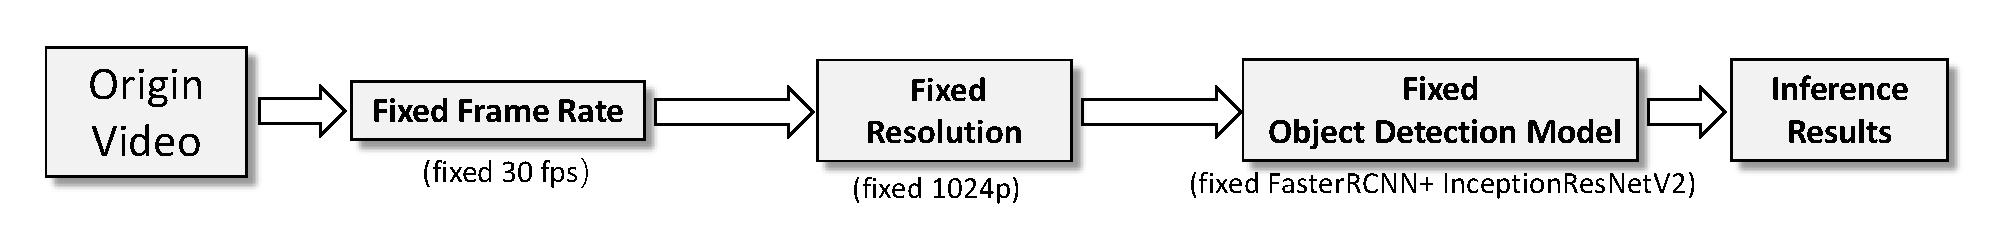
\includegraphics[width=0.9\linewidth]{figures/static_framework.pdf}}
		\begin{center}
			{(a) Static configuration solution: fixed configuration for video analytics services}
		\end{center}
		%        \vspace{0.3cm}
	\end{minipage}
	\vfill
	\vspace{0.4cm}
	\begin{minipage}{\linewidth}
		\centerline{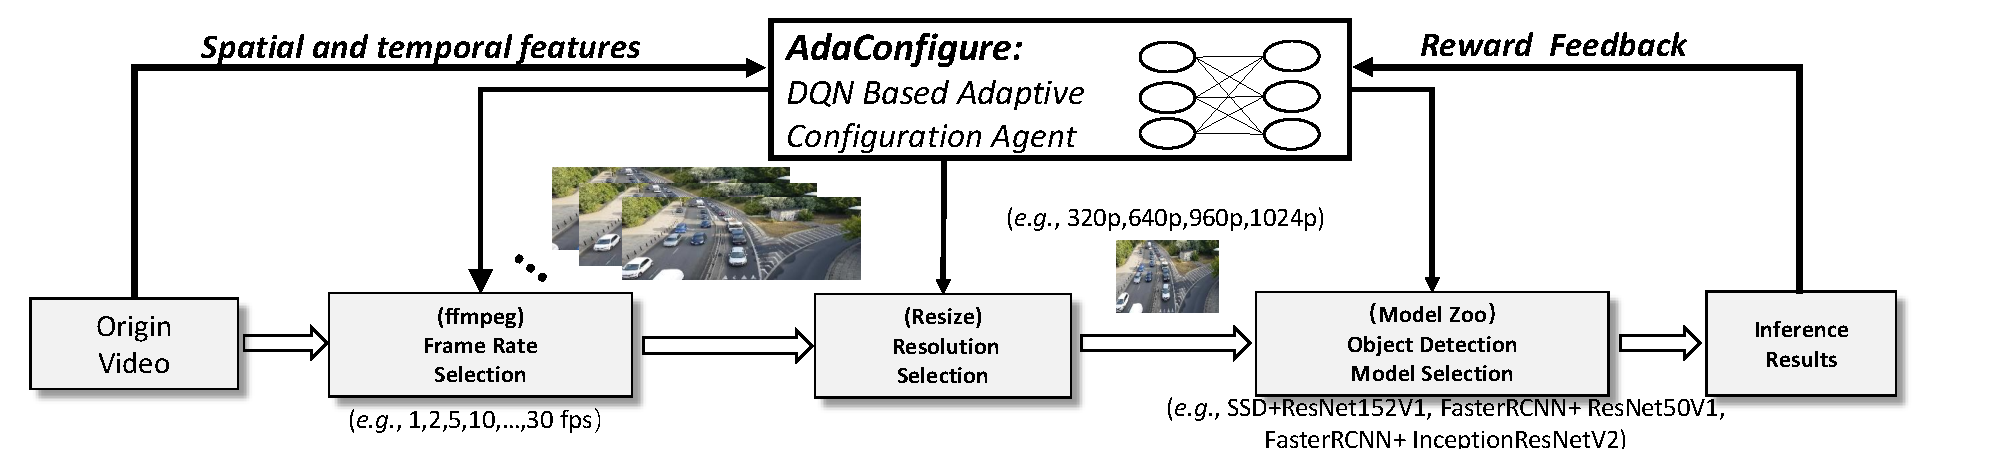
\includegraphics[width=0.9\linewidth]{figures/auto_framework.pdf}}
		\vspace{0.2cm}
		\begin{center}
			{(b) AdaConfigure solution: reinforcement learning-based adaptive configuration framework}
		\end{center}
	\end{minipage}
	%\end{tabular}
	%\vspace{0.1cm}
	\caption{Comparing to the static solution, our solution can adaptively update the configuration strategy based on the object detection model feedback}
	%	\caption{Comparing to the static solution, our solution can update the configuration strategy based on the object detection model feedback}
	\label{fig: framework}
\end{figure*}

\begin{itemize}	
	\item \emph{Choosing the best configuration is a complicated decision-making problem that is challenging to be solved by rules.} The best configuration for video analytics services changes significantly because the exact context of the videos varies over time and across space. For instance, tracking vehicles when traffic moves quickly requires a higher frame rate than when traffic moves slowly. Spatially, the characteristics of video content are different in different locations. For instance, cameras in downtown areas show more cars than the other cameras deployed in the suburbs. It is hard to make an exact rule to choose a configuration for the current context by profiling such complicated video characteristics.
%	but each condition may vary by hour, minute, even second.
	%As a dynamic video analytics configuration %solution
	%application, we target to provide a solution that dynamically picks a configuration according to intrusive dynamics of video contexts, i.e., it can \emph{generate} video analytics configuration for video analytics in a different time.
	
	\item \emph{Adaptive configuration would cause a huge extra overhead.} %The number of possible configurations grows exponentially, 
	There are thousands of configurations can be combined with just a few knobs \cite{jiang2018chameleon}. So exhaustive periodically (e.g., profile once per 4 seconds) configuration to find the best configuration is a highly unrealistic approach because it causes a huge extra overhead, which may exceed the benefits of adaptive configurations. To significantly reduce the resource cost for adaptive configuration profiling requires one solution that automaticly choose a configuration instead of manually trying using various configurations, which is challengling to previous studies including \cite{wang2020jcab,jiang2018chameleon}, since their approaches pay attention to reduce search space algorithm and still try using various configurations to find the best configuration. 
	
	%We leverage a Reinforcement Learning-based agent to adaptively pick the best configuration periodically, dramatically reducing the profiling cost. 
	%How to significantly reduce the resource cost of periodic configuration profiling.
	
	%\item \emph{Lack of well-labeled training data.} In our case, there was no well-marked data that indicated which configuration should be choosed at which time of the video, as is the case with traditional deep learning tasks.%In our problem, one is not provided the well-labeled data on which configuration should be used in which time of the video, as in conventional supervised deep learning tasks. In practice, such a video analytics configuration is usually utilized online, and the solution has to adaptively learn from the video contexts. 
\end{itemize}

%To address the above problems, 
%To address the above complicated decision-making problem and reduce the huge extra overhead of manually trying using various configurations,
%We carefully design an adaptive configuration framework based on reinforcement learning, which is an excellent approach to solve this unsupervised complex-environmental problem. 
In our solution, AutoConfigure can adaptively and automatically select the best configuration according to intrusive dynamics of video contexts, thus solving this difficult optimal configuration decision problem in a low-cost way. To the best of our knowledge, we are the first to propose an adaptive video configuration solution for such problems. 
%that adaptively and automatically chooses a configuration according to the current video context. 
The main contributions of this paper are summarized as follows. 

\begin{itemize}	
	\item We propose a Deep Q-learning Network-based \cite{DQN} agent to adaptively pick the best video analytics configuration according to the characteristics of the video stream. For the agent's state, we extract the spatial and temporal features of the video context, so that the agent can adaptively update configuration over time and achieve a superior performance in the multi-camera situation. 
	
	\item To reduce profiling cost, we leverage a video segmentation strategy and the extremely short choosing action time of agent. In particular, we divide the video into $T$-second intervals as video chunks and use the agent to choose the best configuration for the first t seconds of the video chunk, and then sticks with the chosen configuration for the rest of the video chunk ($T-t$ seconds).
%to capture the characteristics of the video stream with much-reduced computation cost: profiling a segment uses only 0.2-2\% computation resource as compared to a full video.
%	Also, we define the elements of the RL-based approach, such as actions, states, and rewards, to decide the configuration for the current video context.
	
	\item For the agent's reward, we carefully consider both inference accuracy and computation resources to assess each configuration's impact. Also, to meet different accuracy-demand services, we leverage the balance factor in the reward function to train different agents. Our solution can adaptively update configuration strategy over time, and it adaptive to different location-camera inferences and different accuracy-demand services.

% 	First, we design a reinforcement learning-based framework in which an agent adaptively chooses the configuration according to the spatial and temporal features of the current video stream.
	%	 We design an interactive training environment that can be applied to different video analytics applications.
	%	\item We build a reinforcement learning-based framework to train the agent in the above environment. The agent can learn to choose a ``most appropriate'' configuration for each timestamp of video analytics after iteratively interacting with the environment by feeding the carefully designed reward that considers both accuracy and resources.
	
%	\item We leverage dividing video strategy and the extremely short choosing action time of agent to reduce profiling cost. In the evaluation, AdaConfigure achieves 10-35\% higher accuracy with a similar amount of resources or achieves similar accuracy with only 60-90\% of the resources. Our solution proves to be more efficient than static solutions and only creates an overhead of 0.2-2\% to the overall video analytics services.
	
%	\item Our evaluation experiments on object detection task show that our approach outperforms baseline: it achieves 10-35\% higher accuracy with a similar amount of computation resources or achieves similar accuracy with only 60-90% of the computation resource. 
\end{itemize}

%The rest of this paper is organized as follows. We discuss related works in Section \ref{Section: related_works}. We present our framework and detailed design in Section \ref{Section: design}. We present our solution's performance in Section \ref{Section: evaluation} and conclude the paper in Section \ref{Section: conclusion}.

%Since video analytics applications demand intensive computation resources and high accuracy, we pay much attention to the consumption of resources in the calculation process and the inference accuracy. Therefore, the problem that follows is how to balance \emph{resource consumption} and \emph{accuracy}.

%Apparently, choosing different configurations will affect resource consumption and accuracy. When at a fixed frame rate, using a complex model with high resolution can obviously and accurately detect the target object, but it also requires more computing resources. Similarly, when using the same model with the same resolution, choosing a lower resolution can reduce the computing resources, and the subsequent cost is the decline of accuracy. When the target car (object) is large, a smaller model and a lower resolution can meet the accuracy with a considerable reduction of resource consumption, while the target car (object) is small, a more complex model and higher resolution are needed to achieve satisfactory accuracy. And in the case of highway video analytics, the rate of car travel cannot be predicted in advance, so when the car drives slowly (or static) because of the traffic jam, we can choose a lower frame rate (such as 1 FPS) instead of having to use a constant high frame rate throughout the whole video. This can significantly reduce resource consumption but does not affect the accuracy of video analytics. 


%\begin{figure*}[!t]
%	\centerline{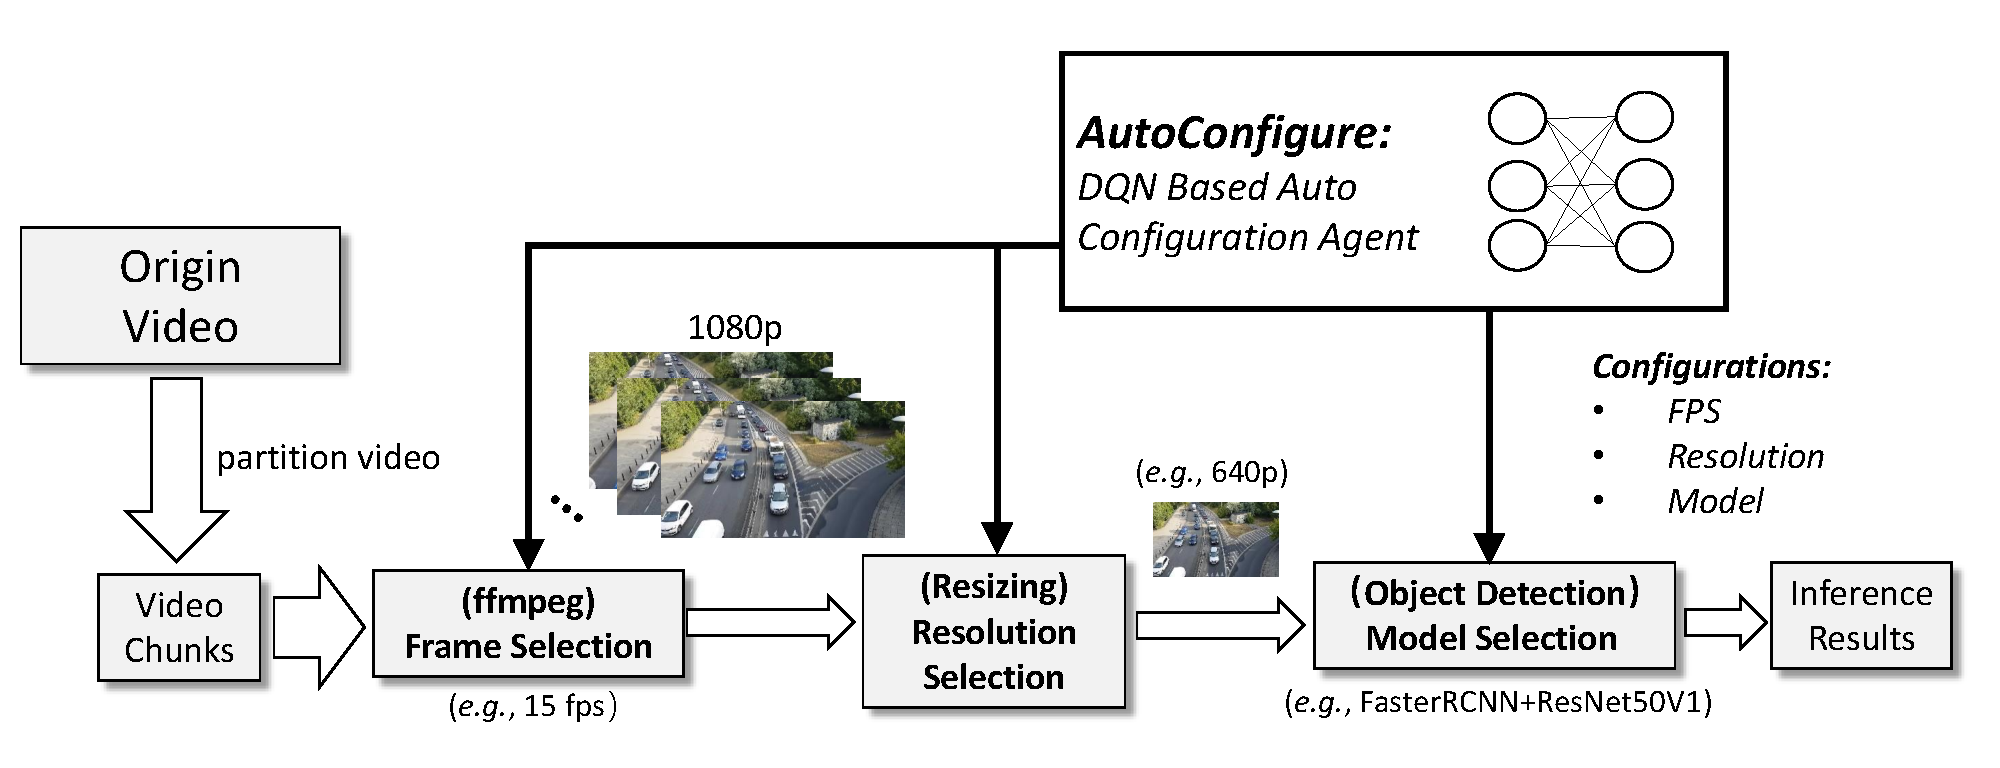
\includegraphics[width=0.9\linewidth]{figures/framework.pdf}}
%	%	\vspace{0.2cm}
%	\caption{Framework of AutoConfigure architecture}
%	\label{fig: framework}
%\end{figure*}

%We use~\autoref{fig2} to support that, the data in this figure come from a real road. It can be found that with the decrease of frame rate, the resource consumption can be significantly reduced, but the reduction of accuracy is partly acceptable.

%As shown in~\autoref{fig1}, at a fixed frame rate, using a complex model with high resolution (such as FasterRCNN+InceptionResnet 1024p) can obviously and accurately detect the target object, but it also requires more computing resources. However, when using the same model, choosing a lower resolution can reduce the computing resources, and the subsequent cost is the decline of accuracy. Another example is that choosing a simple model with low resolution (such as FasterRCNN+ResNet50 640p) can significantly reduce resource consumption, although it reduces the accuracy to some extent.

%\begin{figure}[h]
%\includegraphics[width=9cm,height=5cm]{figures/figure1.pdf}
%\centering
%\caption{The effect of different models and resolutions on accuracy and processing time at a fixed frame rate.}
%\label{fig1}
%\end{figure}
%
%\begin{figure}[h]
%\includegraphics[width=9cm,height=5cm]{figures/figure2.pdf}
%\centering
%\caption{Under the best model, the accuracy and processing time vary with the different frame rate.}
%\label{fig2}
%\end{figure}


%Like figure~\ref{fig: framework}(a), if one just use a unified static configuration solution (i.e.only profiles the processing pipeline to choose the best configuration \emph{once}), the application would either waste resources (by picking an expensive configuration) or sacrifice accuracy (by selecting a cheap configuration).

%Hence, we aim to find a range of ``most appropriate'' configurations that %takes up the
%minimize the consumption of computing resources and is accurate to the desired threshold. On the one hand, like figure~\ref{fig: framework}(a), if one just use a unified static configuration solution (i.e.only profiles the processing pipeline to choose the best configuration \emph{once}), the application would either waste resources (by picking an expensive configuration) or sacrifice accuracy (by selecting a cheap configuration). On the other hand, if one periodically profiles the processing pipeline to find an optimal resource-accuracy \emph{tradeoff} by exhaustive all configurations, it would be prohibitively expensive since the configuration space is extremely large, and thousands of configurations can be combined with just a few knobs. To tackle these challenges, we propose an adaptive configuration approach, AutoConfigure, and the brief framework is shown in Figure~\ref{fig: framework}(b).

%The most intuitive way to solve this problem is to find the best solution by exhaustive all configurations. Still, the number of possible configurations grows exponentially, and thousands of configurations can be combined with just a few knobs, so exhaustive configuration is a highly unrealistic approach.

%For a video analytics application, choosing the ``most appropriate'' configuration is a complicated decision-making problem that is challenging to solve by rules. An adaptive approach is needed to learn from video contexts to decide the best configuration for the current video context. The reinforcement learning method is an excellent way to solve this unsupervised complex-environmental problem. In our solution, we tackle the following design challenges.


%Also, one is not provided the well-labeled data on which configuration should be used at which time of the video, meaning this is an unsupervised learning task.


\section{Related Works}
\label{Section: related_works}

\subsection{Static configuration optimization} 
Several previous papers have considered optimizing video processing pipelines by either adjusting the configuration knobs or training specialized NN models. VideoStorm \cite{zhang2017videostorm} profiles thousands of video analytics queries on live video streams over large clusters, achieving resource-quality tradeoff with multi-dimensional configurations. VideoEdge \cite{hung2018videoedge} introduces \emph{dominant demand} to identify the best tradeoff between multiple resources and accuracy, and narrows the search space by identifying a ``Pareto ban'' of promising configurations. MCDNN \cite{han2016mcdnn} provides a heuristic scheduling algorithm to adaptively select model variants of different accuracy for
deep stream processing under resource constraints. Focus \cite{hsieh2018focus} deconstructs video analytics into two phases, i.e., video ingest and video query. By tuning the share of computing resources of both phases, Focus achieves effective and flexible tradeoff of latency and accuracy of video analytics. These algorithms all profile and optimize video analytics only once at the beginning of the video. They do not handle changes in video stream content. But the optimal configurations do change over time because of the complex and changeable environment.

\subsection{Dynamic configuration optimization}
Some papers study how to dynamically optimize the configuration for video analytics when the video stream content changes.
\cite{shen2017retrain_model} adaptively retrains the NN model to detect the set of popular objects as it changes over time in the video classification task. \cite{yang2019edge_coordinated} proposes an online video quality and computing resource configuration algorithm to gradually learn the optimal configuration strategy, effectively improving the analytic accuracy while providing the low-latency response. INFaaS \cite{romero2019infaas} automatically selects a model, hardware architecture, and any compiler optimizations, and makes scaling and resource allocation decisions when application load varies and the available resources vary over time. JCAB \cite{wang2020jcab} jointly optimizes
configuration adaption and bandwidth allocation to address several critical challenges in edge-based video analytics systems,
including edge capacity limitation, unknown network variation,
intrusive dynamics of video contents. The online algorithm effectively balances analytics accuracy and energy
consumption while keeping low system latency.
 
The closest work to ours is Chameleon \cite{jiang2018chameleon}, which dynamically picks the best configurations for video analytics pipelines, reducing resource consumption
with little degradation in accuracy. They leverage temporal and spatial correlation to amortizes the cost of profiling over time and across multiple cameras, and exploit the knob independence to reduce the search space from exponential to linear. Even the search space is linear, and the profiling cost is still expensive. Such a 24-hours video, Chameleon profiles the configuration space once in every profiling window (16s), it would profile 5400 times. One profiling cost grows linear in the number of configuration knobs and the number of values per knob. The total profiling cost which is equal to one profiling cost multiply the number of profiling (5400) is also significantly high. \textcolor{note}{a little strange, can tangchen help amend?} Our solution called PerConfigure leverages a reinforcement learning-agent to choose the best configuration periodically, significantly reducing the cost of profiling since the choosing time is extremely lower. 
\section{Detailed Design}
\label{Section: design}


\begin{figure*}[!t]
	\centerline{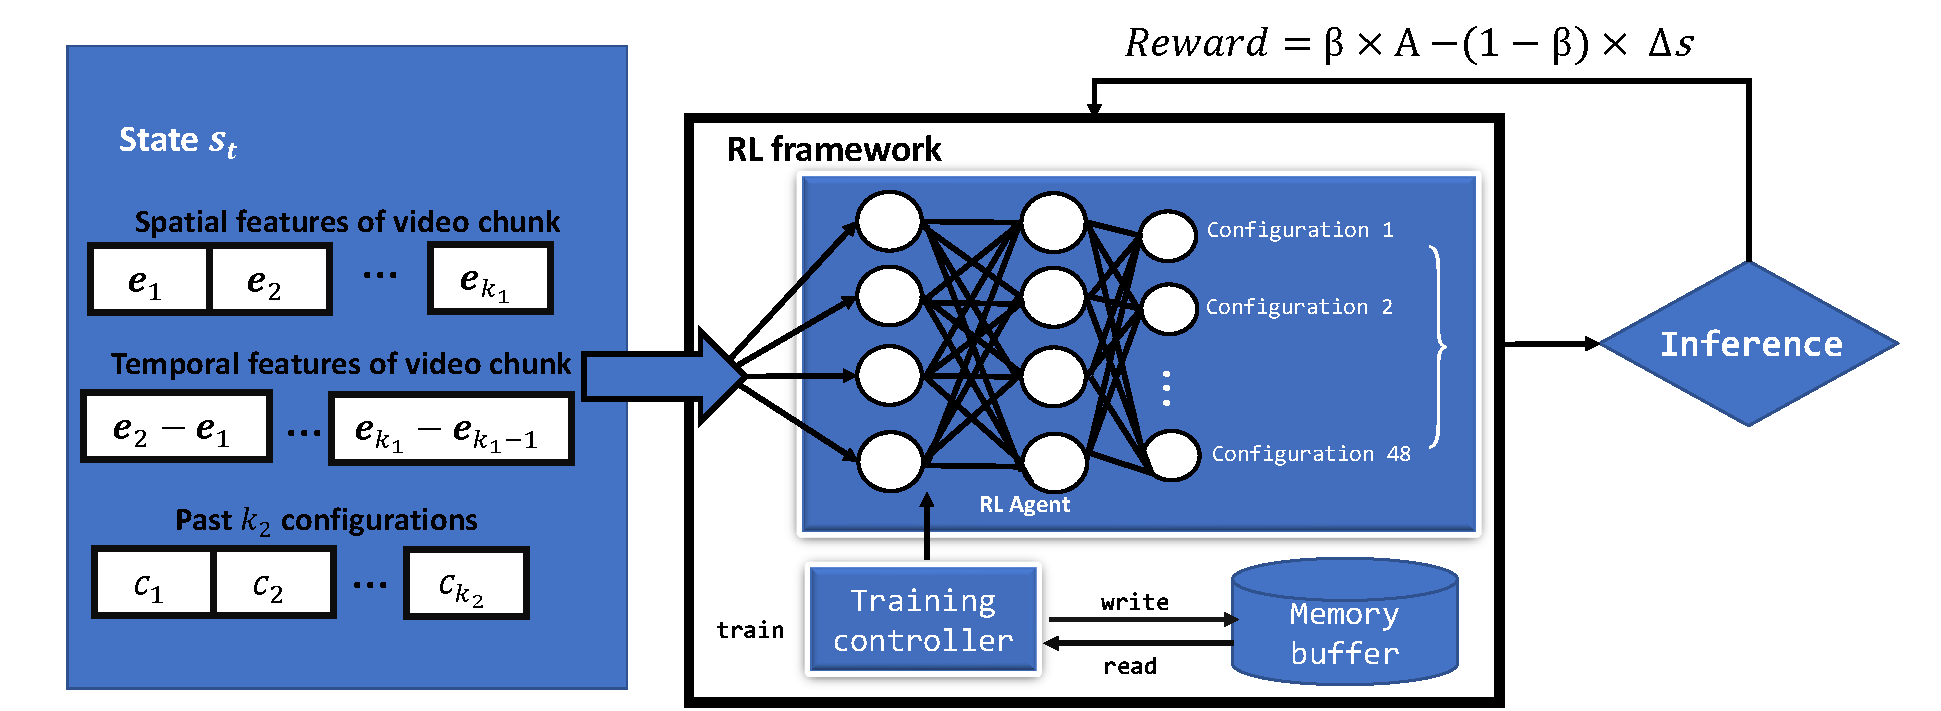
\includegraphics[width=0.9\linewidth]{figures/framework2.pdf}}
	%	\vspace{0.2cm}
	\caption{Applying reinforcement learning to adaptive configuration}
	\label{fig: DQN}
\end{figure*}

Figure~\ref{fig: DQN} summarizes how RL can be applied to the adaptive configuration. Briefly, it is a reinforcement learning-based system to train an agent to choose a proper configuration $ c $ for one video chunk to inference. We discuss the formulation, agent design, reinforcement learning-based framework, reward feedback in the following subsections. We provide experimental details of all the hyperparameters in Section~\ref{Section: experiment}. %% \\

\subsection{Problem Formulation}
\label{subsec: formulation}

To adaptively choose different configuration for video stream, we divides the video into T-second intervals as video chunks, and profiles configurations for each video chunk. Without loss of generality, we denote the object detection service as $ \vec{y}_i = M(x_i) $ that provides a predicted result list $ \vec{y}_i $ for each input video chunk $ x_i $. It has a baseline output $ \vec{y}_{\rm ref} = M(x_{\rm ref}) $ for each input video chunk $ x \in X_{\rm ref} $ using \emph{reference configuration} (the most expensive configuration). We use this $ \vec{y}_{\rm ref} $ as the ground truth label. For each video chunk $ x_c $ that uses a configuration $ c $, the output $ \vec{y}_c = M(x_c) $. Therefore, we have an accuracy metric $ \mathcal{A}_c $ by comparing $ \vec{y}_{\rm ref} $ and $ \vec{y}_c $. In general, we use the F1 score as the accuracy $ \mathcal{A} $, which is the harmonic mean of precision and recall, consistent with prior work~\cite{jiang2018chameleon,kang2017f1_noscope,zhang2017f1_live}. Besides, to compute the accuracy of a frame that was not sampled by $ c $, we use the location of objects from the previous sampled frame. 

For the cost of the object detection service, we use average GPU processing time per frame as the metric of resource consumption. We also denote the metric of resource consumption as $ \hat{s}_{ic} $ that for an input video chunk $ x_i $ and a given configuration $ c $. For a reference configuration $ c_{\rm ref} $, the reference resource consumption is $ \hat{s}_{\rm ref} $.

Initially, the agent tries different configurations $ c $ to obtain inference results image $ x_c $ from input video chunk $ x $. To obtain object detection results $ \{\vec{y}_{\rm ref}, \vec{y}_c\} $, the agent uses the choosen configuration $ c $ and the reference configuration $ x_{\rm ref} $. Comparing the two object detection results $ \{\vec{y}_{\rm ref}, \vec{y}_c\} $ and two resource consumptions $ \{\hat{s}_{\rm ref}, \hat{s}_c\} $, the agent computes the resource consumption ratio $ \Delta s = \frac{\hat{s}_c}{\hat{s}_{\rm ref}} $ and accuracy metric $ \mathcal{A}_c $.

\subsection{RL Agent Design}

The RL agent is expected to give a proper configuration $ c $ for minimizing the resource consumption $ \hat{s}_c $ while keeping the accuracy $ \mathcal{A} $. For the RL agent, the input features are continuous numerical vectors, and the expected output is discrete compression quality level $ c $. Therefore we can use the Deep Q-learning Network \cite{DQN} as the RL agent. But the naive Deep Q-learning Network can not work well in this task because the state space of reinforcement learning is too large if we directly treat video chunk as the input, making the RL agent extremely difficult to converge.  

%But the naive Deep Q-learning Network can not work well in this task because the state space of reinforcement learning is too large if we directly treat video chunk as the input. To preserve enough details, we have to add many layers and nodes to the neural network, making the RL agent extremely difficult to converge. 

%because of the following challenges: %% \\
%
%\begin{itemize}
%	\item The state space of reinforcement learning is too large. To preserve enough details, we have to add many layers and nodes to the neural network, making the RL agent extremely difficult to converge. 
%	\item It takes a long time to train one step in a large inference neural network, making the training process too time-consuming.
%	\item The RL agent starts training from random trials and learns afterward from the reward feedback. When training from a randomly initialized neural network, the reward feedback is very sparse, making it difficult for the agent to learn.
%\end{itemize}

To address this challenges, we leverage FFmpeg \cite{FFmpeg} to extract the top $k_1$ representative images from each chunk as spatial features of video chunk. We use a pre-trained small neural network to extract the structural information embeddings $ \{e_1,e_2,...,e_{k_1}\} $ of the images to reduce the input dimension and accelerate the training procedure. This is a commonly used strategy in training a deep neural network~\cite{finetunning,finetunning2}. In this work, we use the early convolution layers of MobileNetV2~\cite{MobileNetV2} as the image feature extractor $ \mathcal{E}(\cdot) $ for its efficiency in image classification. To extract the temporal features of video chunk, we obtain $ \{\hat{e}_1,\hat{e}_2,...,\hat{e}_{{k_1}-1}\} $ by each embedding subtracting previous embedding. Besides, we record the last $k_2$ configurations $ \{c_1,c_2,...,c_{k_2}\} $. To Solve that vectors of different lengths are not conducive to input to the neural network, we use fully connected layer to transform the spatial embedding $ \{e_1,e_2,...,e_{k_1}\} $, temporal embedding $ \{\hat{e}_1,\hat{e}_2,...,\hat{e}_{{k_1}-1}\} $, and recent configuration $ \{c_1,c_2,...,c_{k_2}\} $ to the fixed length vector, similar to the work~\cite{pensieve}. We formulate the fixed length vector $ s $ as \emph{states} and the configuration $ c $ as discrete \emph{actions}.

\subsection{Reinforcement Learning-based Framework}

In our system, we define 48 discrete actions to indicate 48 configuration, and the specific configurations are provided in Section~\ref{subsec: configuration}. We denote the \emph{action-value function} as $ Q(s, c; \theta) $ and the optimal compression quality level at time $ t $ as $  c_t = {\rm argmax}_cQ(s, c; \theta) $ where $ \theta $ indicates the parameters of the Deep Q-learning Network $ \phi $. In such reinforcement learning formulation, the training phase is to minimize the loss function $ L_i(\theta_i) = \mathbb{E}_{s, c \sim \rho (\cdot)}\Big[\big(y_i - Q(s, c; \theta_i)\big)^2 \Big] $ that changes at each iteration $ i $ where target $ y_i = \mathbb{E}_{s' \sim \{\mathcal{X}, M\}} \big[ r + \gamma \max_{c'} Q(s', c'; \theta_{i-1}) \mid s, c \big] $. Especially, $ r $ is the reward feedback, and $ \rho(s, c) $ is a probability distribution over state  $ s $ and the configuration $ c $~\cite{DQN}. When minimizing the distance of \emph{action-value function}'s output $ Q(\cdot) $ and target $ y_i $, the \emph{action-value function} $ Q(\cdot) $ outputs a more accurate estimation of an action. 

In the training phase, the RL agent firstly using an $\epsilon-$greedy method to take some random trials to observe the environment's reaction and decreases the randomness when training afterward. In iteration $t$, we input state $s_t $ to neural network $ \phi $. The RL agent $\phi$ generates a specific configuration $c_t$. The framework processes the video chunk $x_t$ using configuration $c_t$ to inference object detection services and obtains reward $r_t$. Then the framework obtains the next video chunk $x_{t+1}$ and generates the next state $ s_{t+1} $. The framework stores transition $(s_t, c_t, r_t, s_{t+1})$ in a memory buffer $\mathcal{D}$. Especially, the transition $(s_t, c_t, r_t, s_{t+1} )$ is uesd to compute the loss function. All transitions are saved into a memory buffer $ \mathcal{D} $, and the agent learns to optimize its \emph{action} by minimizing the loss function $ L $ on a mini-batch from $ \mathcal{D} $. The training procedure would converge when the agent's randomness keeps decaying. Finally, the agent's action is based on its historical ``optimal'' experiences. The training procedure is presented in Algorithm~\ref{alg: rl-train}.

\begin{algorithm}[!t]
		\caption{Training RL agent $ \phi $} %in environment $ \{\mathcal{X}, M\} $}
		\label{alg: rl-train}
		\begin{algorithmic}[1]	
			\STATE Initialize action-value function $ Q $ with random weights $ \theta $, replay memory buffer $ \mathcal{D} $ and state $ s_1 $				
			\FOR {$t \in 1,2,\cdots, K$}
			\STATE \textbf{1) Exploration}
			\STATE With probability $\epsilon$:
			\STATE \hspace{1em} $c_t \leftarrow$ a random valid value 
			\STATE Otherwise:
			\STATE \hspace{1em} $ c_t \leftarrow {\rm argmax}_cQ(s_t, c; \theta) $ 

			\STATE \textbf{2) Reward calcuation} 
			\STATE Process video chunk $ x_t $ using configuration $ c_t $ to inference
			\STATE Obtain $ (\vec{y}_{\rm ref}, \vec{y}_c) $ from the object detection service
			\STATE Compute reward $ r \leftarrow R(\Delta s, \mathcal{A}_c) $ according to \ref{subsec: reward} Reward Feedback Design 
			\STATE \textbf{3) Gradient descent}
			\STATE Obtain next video chunk $ x_{t+1} $
			\STATE Generate next state $ s_{t+1} $
			\STATE $ \mathcal{D} \leftarrow \mathcal{D} \bigcup \{(s_t, c_t, r_t, s_{t+1} \} $
			\STATE Sample a randomly mini-batch of transitions $ (s_j, c_j, r_j, s_{j+1}) $ from memory buffer $ \mathcal{D} $
			\STATE $ y_j \leftarrow r_j + \gamma \max_{c'}Q(s_{j+1}, c'; \theta) $
			\STATE Perform a gradient descent step on $ \big(y_j - Q(s_j, c_j; \theta)\big)^2 $ according to~\cite{DQN}
			\ENDFOR
		\end{algorithmic}
\end{algorithm}

\subsection{Reward Feedback Design}
\label{subsec: reward}

In our solution, the agent is trained by the reward feedback. In the above formulation, we define resource consumption rate $ \Delta s = \frac{\hat{s}_c}{\hat{s}_{\rm ref}} $ and accuracy metric $ \mathcal{A}_c $ at configuration $ c $. Basically, we want the agent to choose a proper configuration for minimizing the resource consumption while remaining acceptable accuracy. Therefore the overall reward $ r $ should be positively correlated with the accuracy $ \mathcal{A} $ while negatively with the resource consumption ratio $ \Delta s $. We introduce a balance factor $ \beta $ to form a linear combination $ r = \beta \mathcal{A} - (1-\beta) \Delta s  $ as the \emph{reward function} $ R(\Delta s, \mathcal{A}) $. %% \\

\section{Evaluation}
\label{Section: evaluation}

\subsection{Experiment Setup}

\subsection{some results}

%\begin{table}[!t]
%\begin{table}[H]
%	\centering
%	%     \begin{tabular}{lll}
%	\resizebox{0.5\textwidth}{!}{
%	\begin{tabular}{lcc}
%		\toprule
%		Model and Image size & Inference time & Accuracy  \\ \midrule
%		SSD MobileNetV2 320p          & 49.5 ms  &  xxx            \\
%		SSD MobileNetV2 640p          & 58.5 ms  &  0.494            \\
%		SSD ResNet152V1 640p          & 100 ms  &  0.579            \\
%		SSD ResNet152V1 1024p          & 182.3 ms  &  0.614            \\
%		FasterRCNN ResNet50V1 640p          & 106.4 ms  &  0.637            \\
%		FasterRCNN ResNet50V1 1024p          & 120.5 ms  &  0.786           \\
%		FasterRCNN InceptionResNetV2 640p          & 361.8 ms  &  0.734            \\
%		FasterRCNN InceptionResNetV2 1024p          & 418.4 ms  &  1            \\
%		\bottomrule
%	\end{tabular}}
%	\caption{Inference time and F1 for different models and resolutions}
%	\label{tab: latency-overhead}
%	% \vspace{-0.5cm}
%\end{table}

%\begin{table}[!t]
\begin{table}[H]
	\centering
	%     \begin{tabular}{lll}
	\resizebox{0.5\textwidth}{!}{
		\begin{tabular}{lcc}
			\toprule
			Model and Image size & Inference time & Accuracy  \\ \midrule
			SSD MobileNetV2 320p          & 49.5 ms  &  xxx            \\
			SSD MobileNetV2 640p          & 58.5 ms  &  0.753            \\
			SSD ResNet152V1 640p          & 100 ms  &  0.886            \\
			SSD ResNet152V1 1024p          & 182.3 ms  &  0.942            \\
			FasterRCNN ResNet50V1 640p          & 106.4 ms  &  0.889            \\
			FasterRCNN ResNet50V1 1024p          & 120.5 ms  &  0.98           \\
			FasterRCNN InceptionResNetV2 640p          & 361.8 ms  &  0.965            \\
			FasterRCNN InceptionResNetV2 1024p          & 418.4 ms  &  1            \\
			\bottomrule
	\end{tabular}}
	\caption{Inference time and F1 for different models and resolutions}
	\label{tab: latency-overhead}
	% \vspace{-0.5cm}
\end{table}
\section{Conclusion}
\label{Section: conclusion}

This paper proposes a reinforcement learning (RL)-based automatic video analytics configuration framework, AutoConfigure. Our solution can adapt the best configuration to intrusive dynamics of video contexts, meaning that it can periodically choose the proper configuration for the current video chunk according to the spatial and temporal correlation of video contexts. In the evaluation, AutoConfigure achieves 10-35\% higher accuracy with a similar amount of resources or achieves similar accuracy with only 50-85\% of the resources. AutoConfigure proves to be more efficient than static solutions and only creates an overhead of 0.1-1\% to the overall video analytics services.

%\section{Copyright}
%All papers submitted for publication by AAAI Press must be accompanied by a valid signed copyright form. There are no exceptions to this requirement. You must send us the original version of this form. However, to meet the deadline, you may fax (1-650-321-4457) or scan and e-mail the form (pubforms20@aaai.org) to AAAI by the submission deadline, and then mail the original via postal mail to the AAAI office. If you fail to send in a signed copyright or permission form, we will be unable to publish your paper. There are \textbf{no exceptions} to this policy.You will find PDF versions of the AAAI copyright and permission to distribute forms in the AAAI AuthorKit.
%
%\section{Formatting Requirements in Brief}
%We need source and PDF files that can be used in a variety of ways and can be output on a variety of devices. The design and appearance of the paper is strictly governed by the aaai style file (aaai20.sty). 
%\textbf{You must not make any changes to the aaai style file, nor use any commands, packages, style files, or macros within your own paper that alter that design, including, but not limited to spacing, floats, margins, fonts, font size, and appearance.} AAAI imposes requirements on your source and PDF files that must be followed. Most of these requirements are based on our efforts to standardize conference manuscript properties and layout. All papers submitted to AAAI for publication will be recompiled for standardization purposes. Consequently, every paper submission must comply with the following requirements:
%
%\begin{quote}
%\begin{itemize}
%\item Your .tex file must compile in PDF\LaTeX{} --- ( you may not include .ps or .eps figure files.)
%\item All fonts must be embedded in the PDF file --- including includes your figures.
%\item Modifications to the style file, whether directly or via commands in your document may not ever be made, most especially when made in an effort to avoid extra page charges or make your paper fit in a specific number of pages.
%\item No type 3 fonts may be used (even in illustrations).
%\item You may not alter the spacing above and below captions, figures, headings, and subheadings.
%\item You may not alter the font sizes of text elements, footnotes, heading elements, captions, or title information (for references and mathematics, please see the the limited exceptions provided herein).
%\item You may not alter the line spacing of text.
%\item Your title must follow Title Case capitalization rules (not sentence case).
%\item Your .tex file must include completed metadata to pass-through to the PDF (see PDFINFO below)
%\item \LaTeX{} documents must use the Times or Nimbus font package (you may not use Computer Modern for the text of your paper).
%\item No \LaTeX{} 209 documents may be used or submitted.
%\item Your source must not require use of fonts for non-Roman alphabets within the text itself. If your paper includes symbols in other languages (such as, but not limited to, Arabic, Chinese, Hebrew, Japanese, Thai, Russian and other Cyrillic languages), you must restrict their use to bit-mapped figures. Fonts that require non-English language support (CID and Identity-H) must be converted to outlines or 300 dpi bitmap or removed from the document (even if they are in a graphics file embedded in the document). 
%\item Two-column format in AAAI style is required for all papers.
%\item The paper size for final submission must be US letter without exception.
%\item The source file must exactly match the PDF.
%\item The document margins may not be exceeded (no overfull boxes).
%\item The number of pages and the file size must be as specified for your event.
%\item No document may be password protected.
%\item Neither the PDFs nor the source may contain any embedded links or bookmarks (no hyperref or navigator packages).
%\item Your source and PDF must not have any page numbers, footers, or headers (no pagestyle commands).
%\item Your PDF must be compatible with Acrobat 5 or higher.
%\item Your \LaTeX{} source file (excluding references) must consist of a \textbf{single} file (use of the ``input" command is not allowed.
%\item Your graphics must be sized appropriately outside of \LaTeX{} (do not use the ``clip" or ``trim'' command) .
%\end{itemize}
%\end{quote}
%
%If you do not follow these requirements, you will be required to correct the deficiencies and resubmit the paper. A resubmission fee will apply.
%
%\section{What Files to Submit}
%You must submit the following items to ensure that your paper is published:
%\begin{itemize}
%\item A fully-compliant PDF file that includes PDF metadata.
%\item Your \LaTeX{} source file submitted as a \textbf{single} .tex file (do not use the ``input" command to include sections of your paper --- every section must be in the single source file). (The only allowable exception is .bib file, which should be included separately). 
%\item The bibliography (.bib) file(s).
%\item Your source must compile on our system, which includes only standard \LaTeX{} 2019 TeXLive support files. 
%\item Only the graphics files used in compiling paper.
%\item The \LaTeX{}-generated files (e.g. .aux,  .bbl file, PDF, etc.).
%\end{itemize}
%
%Your \LaTeX{} source will be reviewed and recompiled on our system (if it does not compile, you will be required to resubmit, which will incur fees). \textbf{Do not submit your source in multiple text files.} Your single \LaTeX{} source file must include all your text, your bibliography (formatted using aaai.bst), and any custom macros. 
%
%Your files should work without any supporting files (other than the program itself) on any computer with a standard \LaTeX{} distribution. 
%
%\textbf{Do not send files that are not actually used in the paper.} We don't want you to send us any files not needed for compiling your paper, including, for example, this instructions file, unused graphics files, style files, additional material sent for the purpose of the paper review, and so forth.
%
%\textbf{Do not send supporting files that are not actually used in the paper.} We don't want you to send us any files not needed for compiling your paper, including, for example, this instructions file, unused graphics files, style files, additional material sent for the purpose of the paper review, and so forth.
%
%\textbf{Obsolete style files.} The commands for some common packages (such as some used for algorithms), may have changed. Please be certain that you are not compiling your paper using old or obsolete style files. 
%\textbf{Final Archive.} Place your PDF and source files in a single archive which should be compressed using .zip. The final file size may not exceed 10 MB.
%Name your source file with the last (family) name of the first author, even if that is not you.
%
%
%\section{Using \LaTeX{} to Format Your Paper}
%
%The latest version of the AAAI style file is available on AAAI's website. Download this file and place it in the \TeX\ search path. Placing it in the same directory as the paper should also work. You must download the latest version of the complete AAAI Author Kit so that you will have the latest instruction set and style file.
%
%\subsection{Document Preamble}
%
%In the \LaTeX{} source for your paper, you \textbf{must} place the following lines as shown in the example in this subsection. This command set-up is for three authors. Add or subtract author and address lines as necessary, and uncomment the portions that apply to you. In most instances, this is all you need to do to format your paper in the Times font. The helvet package will cause Helvetica to be used for sans serif. These files are part of the PSNFSS2e package, which is freely available from many Internet sites (and is often part of a standard installation).
%
%Leave the setcounter for section number depth commented out and set at 0 unless you want to add section numbers to your paper. If you do add section numbers, you must uncomment this line and change the number to 1 (for section numbers), or 2 (for section and subsection numbers). The style file will not work properly with numbering of subsubsections, so do not use a number higher than 2.
%
%If (and only if) your author title information will not fit within the specified height allowed, put \textbackslash setlength \textbackslash titlebox{2.5in} in your preamble. Increase the height until the height error disappears from your log. You may not use the \textbackslash setlength command elsewhere in your paper, and it may not be used to reduce the height of the author-title box.
%
%\subsubsection{The Following Must Appear in Your Preamble}
%\begin{quote}
%\begin{scriptsize}\begin{verbatim}
%\documentclass[letterpaper]{article}
%\usepackage{aaai20}
%\usepackage{times}
%\usepackage{helvet}
%\usepackage{courier}
%\usepackage[hyphens]{url} 
%\usepackage{graphicx}
%\urlstyle{rm}
%\def\UrlFont{\rm}
%\usepackage{graphicx}
%\frenchspacing
%\setlength{\pdfpagewidth}{8.5in}
%\setlength{\pdfpageheight}{11in}
%% Add additional packages here, but check 
%% the list of disallowed packages 
%% (including, but not limited to
%% authblk, caption, CJK, float, fullpage, geometry, 
%% hyperref, layout, nameref, natbib, savetrees, 
%% setspace, titlesec, tocbibind, ulem)
%% and illegal commands provided in the 
%% common formatting errors document
%% included in the  Author Kit before doing so. 
%%
%% PDFINFO
%% You are required to complete the following
%% for pass-through to the PDF. 
%% No LaTeX commands of any kind may be
%% entered. The parentheses and spaces 
%% are an integral part of the 
%% pdfinfo script and must not be removed.
%%
%\pdfinfo{
%/Title (Type Your Paper Title Here in Mixed Case)
%/Author (John Doe, Jane Doe)
%/Keywords (Input your keywords in this optional area)
%}
%%
%% Section Numbers
%% Uncomment if you want to use section numbers
%% and change the 0 to a 1 or 2
%% \setcounter{secnumdepth}{0}
%
%% Title and Author Information Must Immediately Follow
%% the pdfinfo within the preamble
%%
%\title{Title}\\
%\author\{Author 1 \ and Author 2\\
%Address line\\
%Address line\\
%\ And\\
%Author 3\\
%Address line\\
%Address line
%}\\
%\end{verbatim}\end{scriptsize}
%\end{quote}
%
%\subsection{Preparing Your Paper}
%
%After the preamble above, you should prepare your paper as follows:
%\begin{quote}
%\begin{scriptsize}\begin{verbatim}
%%
%\begin{document}
%\maketitle
%\begin{abstract}
%%...
%\end{abstract}\end{verbatim}\end{scriptsize}
%\end{quote}
%
%\subsubsection{The Following Must Conclude Your Document}
%\begin{quote}
%\begin{scriptsize}\begin{verbatim}
%% References and End of Paper
%% These lines must be placed at the end of your paper
%\bibliography{Bibliography-File}
%\bibliographystyle{aaai}
%\end{document}
%\end{verbatim}\end{scriptsize}
%\end{quote}
%
%\subsection{Inserting Document Metadata with \LaTeX{}}
%PDF files contain document summary information that enables us to create an Acrobat index (pdx) file, and also allows search engines to locate and present your paper more accurately. \textit{Document metadata for author and title are REQUIRED.} You may not apply any script or macro to implementation of the title, author, and metadata information in your paper.
%
%\textit{Important:} Do not include \textit{any} \LaTeX{} code or nonascii characters (including accented characters) in the metadata. The data in the metadata must be completely plain ascii. It may not include slashes, accents, linebreaks, unicode, or any \LaTeX{} commands. Type the title exactly as it appears on the paper (minus all formatting). Input the author names in the order in which they appear on the paper (minus all accents), separating each author by a comma. You may also include keywords in the optional Keywords field.
%
%\begin{quote}
%\begin{scriptsize}\begin{verbatim}
%\begin{document}\\
%\maketitle\\
%...\\
%\bibliography{Bibliography-File}\\
%\bibliographystyle{aaai}\\
%\end{document}\\
%\end{verbatim}\end{scriptsize}
%\end{quote}
%
%\subsection{Commands and Packages That May Not Be Used}
%\begin{table*}[t]
%\centering
%\caption{Commands that must not be used}\smallskip
%\begin{tabular}{l|l|l|l}
%\textbackslash abovecaption & 
%\textbackslash abovedisplay & 
%\textbackslash addevensidemargin & 
%\textbackslash addsidemargin \\ 
%\textbackslash addtolength & 
%\textbackslash baselinestretch & 
%\textbackslash belowcaption & 
%\textbackslash belowdisplay \\ 
%\textbackslash break &
%\textbackslash clearpage & 
%\textbackslash clip & 
%\textbackslash columnsep \\ 
%\textbackslash float & 
%\textbackslash input & 
%\textbackslash input & 
%\textbackslash linespread \\ 
%\textbackslash newpage &
%\textbackslash pagebreak & 
%\textbackslash renewcommand & 
%\textbackslash setlength \\ 
%\textbackslash text height & 
%\textbackslash tiny & 
%\textbackslash top margin & 
%\textbackslash trim \\ 
%\textbackslash vskip\{- & 
%\textbackslash vspace\{- \\ 
%\end{tabular}
%%}
%\label{table1}
%\end{table*}
%
%\begin{table}[t]
%\caption{LaTeX style packages that must not be used.}\smallskip
%\centering
%%\resizebox{.95\columnwidth}{!}{
%\smallskip\begin{tabular}{l|l|l|l}
%authblk & babel & caption & cjk\\
%dvips & epsf & epsfig & euler\\
%float & fullpage & geometry & graphics\\
%hyperref & layout & linespread & lmodern\\
%maltepaper & natbib & navigator & pdfcomment\\
%pgfplots & psfig & pstricks & t1enc \\
%titlesec & tocbind & ulem\\
%\end{tabular}
%\label{table2}
%\end{table}
%
%There are a number of packages, commands, scripts, and macros that are incompatable with aaai20.sty. The common ones are listed in tables \ref{table1} and \ref{table2}. Generally, if a command, package, script, or macro alters floats, margins, fonts, sizing, linespacing, or the presentation of the references and citations, it is unacceptable. Note that negative vskip and vspace may not be used except in certain rare occurances, and may never be used around tables, figures, captions, sections, subsections, subsections, or references. 
%
%
%\subsection{Page Breaks}
%For your final camera ready copy, you must not use any page break commands. References must flow directly after the text without breaks. Note that some conferences require references to be on a separate page during the review process. AAAI Press, however, does not require this condition for the final paper. 
%
%
%\subsection{Paper Size, Margins, and Column Width}
%Papers must be formatted to print in two-column format on 8.5 x 11 inch US letter-sized paper. The margins must be exactly as follows: 
%\begin{itemize}
%\item Top margin: .75 inches
%\item Left margin: .75 inches
%\item Right margin: .75 inches
%\item Bottom margin: 1.25 inches
%\end{itemize} 
%
%
%The default paper size in most installations of \LaTeX{} is A4. However, because we require that your electronic paper be formatted in US letter size, the preamble we have provided includes commands that alter the default to US letter size. Please note that using any other package to alter page size (such as, but not limited to the Geometry package) will result in your final paper being returned to you for correction and payment of a resubmission fee. 
%
%
%\subsubsection{Column Width and Margins.}
%To ensure maximum readability, your paper must include two columns. Each column should be 3.3 inches wide (slightly more than 3.25 inches), with a .375 inch (.952 cm) gutter of white space between the two columns. The aaai20.sty file will automatically create these columns for you. 
%
%\subsection{Overlength Papers}
%If your paper is too long, turn on \textbackslash frenchspacing, which will reduce the space after periods. Next, shrink the size of your graphics. Use \textbackslash centering instead of \textbackslash begin\{center\} in your figure environment. For mathematical environments, you may reduce fontsize {\bf but not below 6.5 point}. You may also alter the size of your bibliography and tables by inserting \textbackslash fontsize\{9.5pt\}\{10.5pt\} \textbackslash selectfont
%right before the bibliography (the minimum size is \textbackslash fontsize\{9.0pt\}\{10.0pt\}. You may not use any commands that further reduce point size. Be careful when scaling tables and figures. Tables that do not fit in a single column, even after the font size reduction to 9 point, must be placed across double columns. If your table won't fit within the margins even in double columns, you must split it. We will not accept single (or double) column tables that have been scaled to anything below 9 point. 
%
%
%Commands that alter page layout are forbidden. These include \textbackslash columnsep, \textbackslash topmargin, \textbackslash topskip, \textbackslash textheight, \textbackslash textwidth, \textbackslash oddsidemargin, and \textbackslash evensizemargin (this list is not exhaustive). If you alter page layout, you will be required to pay the page fee \textit{plus} a reformatting fee. Other commands that are questionable and may cause your paper to be rejected include \textbackslash parindent, and \textbackslash parskip. Commands that alter the space between sections are forbidden. The title sec package is not allowed. Regardless of the above, if your paper is obviously ``squeezed" it is not going to to be accepted. Options for reducing the length of a paper include reducing the size of your graphics, cutting text, or paying the extra page charge (if it is offered). 
%
%\subsection{Figures}
%Your paper must compile in PDF\LaTeX{}. Consequently, all your figures must be .jpg, .png, or .pdf. You may not use the .gif (the resolution is too low), .ps, or .eps file format for your figures.
%
%If you normally create your figures using pgfplots, please create the figures first, and then import them as pdfs with proper bounding boxes, as the bounding and trim boxes created by pfgplots are fragile, and not valid.
%
%When you include your figures, you must crop them \textbf{outside} of \LaTeX{}. The command \textbackslash includegraphics*[clip=true, viewport 0 0 10 10]{...} might result in a PDF that looks great, but the image is \textbf{not really cropped.} The full image can reappear (and obscure whatever it is overlapping) when page numbers are applied or color space is standardized. Figures \ref{fig1}, and \ref{fig2} display some unwanted results that often occur.
%
%Do not use minipage to group figures. Additionally, the font and size of figure captions must be 10 point roman. Do not make them smaller, bold, or italic. (Individual words may be italicized if the context requires differentiation.)
%
%\begin{figure}[t]
%\centering
%\includegraphics[width=0.9\columnwidth]{figure1} % Reduce the figure size so that it is slightly narrower than the column. Don't use precise values for figure width.This setup will avoid overfull boxes. 
%\caption{Using the trim and clip commands produces fragile layers that can result in disasters (like this one from an actual paper) when the color space is corrected or the PDF combined with others for the final proceedings. Crop your figures properly in a graphics program -- not in LaTeX}
%\label{fig1}
%\end{figure}
%
%\begin{figure*}[t]
%\centering
%\includegraphics[width=0.8\textwidth]{figure2} % Reduce the figure size so that it is slightly narrower than the column.
%\caption{Adjusting the bounding box instead of actually removing the unwanted data resulted multiple layers in this paper. It also needlessly increased the PDF size. In this case, the size of the unwanted layer doubled the paper's size, and produced the following surprising results in final production. Crop your figures properly in a graphics program. Don't just alter the bounding box.}
%\label{fig2}
%\end{figure*}
%
%% Using the \centering command instead of \begin{center} ... \end{center} will save space
%% Positioning your figure at the top of the page will save space and make the paper more readable
%% Using 0.95\columnwidth in conjunction with the 
%
%\subsection{Type Font and Size}
%Your paper must be formatted in Times Roman or Nimbus. We will not accept papers formatted using Computer Modern or Palatino or some other font as the text or heading typeface. Sans serif, when used, should be Courier. Use Symbol or Lucida or Computer Modern for \textit{mathematics only. } 
%
%Do not use type 3 fonts for any portion of your paper, including graphics. Type 3 bitmapped fonts are designed for fixed resolution printers. Most print at 300 dpi even if the printer resolution is 1200 dpi or higher. They also often cause high resolution imagesetter devices and our PDF indexing software to crash. Consequently, AAAI will not accept electronic files containing obsolete type 3 fonts. Files containing those fonts (even in graphics) will be rejected. 
%
%Fortunately, there are effective workarounds that will prevent your file from embedding type 3 bitmapped fonts. The easiest workaround is to use the required times, helvet, and courier packages with \LaTeX{}2e. (Note that papers formatted in this way will still use Computer Modern for the mathematics. To make the math look good, you'll either have to use Symbol or Lucida, or you will need to install type 1 Computer Modern fonts --- for more on these fonts, see the section ``Obtaining Type 1 Computer Modern.")
%
%If you are unsure if your paper contains type 3 fonts, view the PDF in Acrobat Reader. The Properties/Fonts window will display the font name, font type, and encoding properties of all the fonts in the document. If you are unsure if your graphics contain type 3 fonts (and they are PostScript or encapsulated PostScript documents), create PDF versions of them, and consult the properties window in Acrobat Reader. 
%
%The default size for your type must be ten-point with twelve-point leading (line spacing). Start all pages (except the first) directly under the top margin. (See the next section for instructions on formatting the title page.) Indent ten points when beginning a new paragraph, unless the paragraph begins directly below a heading or subheading.
%
%
%\subsubsection{Obtaining Type 1 Computer Modern for \LaTeX{}.}
%
%If you use Computer Modern for the mathematics in your paper (you cannot use it for the text) you may need to download type 1 Computer fonts. They are available without charge from the American Mathematical Society:
%http://www.ams.org/tex/type1-fonts.html. 
%
%\subsubsection{Nonroman Fonts}
%If your paper includes symbols in other languages (such as, but not limited to, Arabic, Chinese, Hebrew, Japanese, Thai, Russian and other Cyrillic languages), you must restrict their use to bit-mapped figures. 
%
%\subsection{Title and Authors}
%Your title must appear in mixed case (nouns, pronouns, and verbs are capitalized) near the top of the first page, centered over both columns in sixteen-point bold type (twenty-four point leading). This style is called ``mixed case," which means that means all verbs (including short verbs like be, is, using,and go), nouns, adverbs, adjectives, and pronouns should be capitalized, (including both words in hyphenated terms), while articles, conjunctions, and prepositions are lower case unless they directly follow a colon or long dash. Author's names should appear below the title of the paper, centered in twelve-point type (with fifteen point leading), along with affiliation(s) and complete address(es) (including electronic mail address if available) in nine-point roman type (the twelve point leading). (If the title is long, or you have many authors, you may reduce the specified point sizes by up to two points.) You should begin the two-column format when you come to the abstract. 
%
%\subsubsection{Formatting Author Information}
%Author information can be set in a number of different styles, depending on the number of authors and the number of affiliations you need to display. In formatting your author information, however, you may not use a table nor may you employ the \textbackslash authorblk.sty package. For several authors from the same institution, please just separate with commas:
%
%\begin{quote}\begin{scriptsize}\begin{verbatim}
%\author{Author 1, ... Author n\\ 
%Address line \\ ... \\ Address line}
%\end{verbatim}\end{scriptsize}\end{quote}
%
%\noindent If the names do not fit well on one line use:
%
%\begin{quote}\begin{scriptsize}\begin{verbatim}
%\author{Author 1} ... \\
%{\bf \Large Author ... Author}\\ 
%Address line \\ ... \\ Address line
%}
%\end{verbatim}\end{scriptsize}\end{quote}
%
%\noindent For two (or three) authors from different institutions, use \textbackslash And:
%
%\begin{quote}\begin{scriptsize}\begin{verbatim}
%\author{Author 1\\ Address line \\ ... \\ Address line 
%\And ... \And Author n\\
%Address line\\ ... \\ Address line}
%\end{verbatim}\end{scriptsize}\end{quote}
%
%\noindent To start a separate ``row" of authors, use \textbackslash AND:
%
%If the title and author information does not fit in the area allocated, place
%\textbackslash setlength\textbackslash titlebox\{\textit{height}\}
%after the \textbackslash documentclass line where \{\textit{height}\} is 2.5in or greater. (This one of the only allowable uses of the setlength command. Check with AAAI Press before using it elsewhere.)
%
%\subsubsection{Formatting Author Information --- Alternative Method}
%If your paper has a large number of authors from different institutions, you may use the following alternative method for displaying the author information.
%
%\begin{quote}\begin{scriptsize}\begin{verbatim}
%\author{AuthorOne},\textsuperscript{\rm 1} 
%AuthorTwo,\textsuperscript{\rm 2}
%AuthorThree,\textsuperscript{\rm 3}
%\\bf \Large AuthorFour,\textsuperscript{\rm 4} 
%AuthorFive, \textsuperscript{\rm 5}\\
%\textsuperscript{\rm 1}AffiliationOne, 
%\textsuperscript{\rm 2}AffiliationTwo, 
%\textsuperscript{\rm 3}AffiliationThree\\
%\textsuperscript{\rm 4}AffiliationFour, 
%\textsuperscript{\rm 5}AffiliationFive 
%\{email, email\}@affiliation.com,
%email@affiliation.com,
%email@affiliation.com, 
%email@affiliation.com
%\end{verbatim}\end{scriptsize}\end{quote}
%
%Note that you should break the author list before it extends into the right column margin. Put a line break, followed by   \textbackslash bf  \textbackslash Large to put the second line of authors in the same font and size as the first line (you may not make authors names smaller to save space.) Affiliations can be broken with a simple line break (\textbackslash  \textbackslash).
%\subsection{\LaTeX{} Copyright Notice}
%The copyright notice automatically appears if you use aaai20.sty. It has been hardcoded and may not be disabled.
%
%\subsection{Credits}
%Any credits to a sponsoring agency should appear in the acknowledgments section, unless the agency requires different placement. If it is necessary to include this information on the front page, use
%\textbackslash thanks in either the \textbackslash author or \textbackslash title commands.
%For example:
%\begin{quote}
%\begin{small}
%\textbackslash title\{Very Important Results in AI\textbackslash thanks\{This work is
% supported by everybody.\}\}
%\end{small}
%\end{quote}
%Multiple \textbackslash thanks commands can be given. Each will result in a separate footnote indication in the author or title with the corresponding text at the botton of the first column of the document. Note that the \textbackslash thanks command is fragile. You will need to use \textbackslash protect.
%
%Please do not include \textbackslash pubnote commands in your document.
%
%\subsection{Abstract}
%Follow the example commands in this document for creation of your abstract. The command \textbackslash begin\{abstract\} will automatically indent the text block. Please do not indent it further. {Do not include references in your abstract!}
%
%\subsection{Page Numbers}
%
%Do not \textbf{ever} print any page numbers on your paper. The use of \textbackslash pagestyle is forbidden.
%
%\subsection{Text }
%The main body of the paper must be formatted in black, ten-point Times Roman with twelve-point leading (line spacing). You may not reduce font size or the linespacing. Commands that alter font size or line spacing (including, but not limited to baselinestretch, baselineshift, linespread, and others) are expressly forbidden. In addition, you may not use color in the text. 
%
%\subsection{Citations}
%Citations within the text should include the author's last name and year, for example (Newell 1980). Append lower-case letters to the year in cases of ambiguity. Multiple authors should be treated as follows: (Feigenbaum and Engelmore 1988) or (Ford, Hayes, and Glymour 1992). In the case of four or more authors, list only the first author, followed by et al. (Ford et al. 1997).
%
%\subsection{Extracts}
%Long quotations and extracts should be indented ten points from the left and right margins. 
%
%\begin{quote}
%This is an example of an extract or quotation. Note the indent on both sides. Quotation marks are not necessary if you offset the text in a block like this, and properly identify and cite the quotation in the text. 
%
%\end{quote}
%
%\subsection{Footnotes}
%Avoid footnotes as much as possible; they interrupt the reading of the text. When essential, they should be consecutively numbered throughout with superscript Arabic numbers. Footnotes should appear at the bottom of the page, separated from the text by a blank line space and a thin, half-point rule. 
%
%\subsection{Headings and Sections}
%When necessary, headings should be used to separate major sections of your paper. Remember, you are writing a short paper, not a lengthy book! An overabundance of headings will tend to make your paper look more like an outline than a paper. The aaai.sty package will create headings for you. Do not alter their size nor their spacing above or below. 
%
%\subsubsection{Section Numbers}
%The use of section numbers in AAAI Press papers is optional. To use section numbers in \LaTeX{}, uncomment the setcounter line in your document preamble and change the 0 to a 1 or 2. Section numbers should not be used in short poster papers.
%
%\subsubsection{Section Headings.}
%Sections should be arranged and headed as follows: 
%
%\subsubsection{Acknowledgments.}
%The acknowledgments section, if included, appears after the main body of text and is headed ``Acknowledgments." This section includes acknowledgments of help from associates and colleagues, credits to sponsoring agencies, financial support, and permission to publish. Please acknowledge other contributors, grant support, and so forth, in this section. Do not put acknowledgments in a footnote on the first page. If your grant agency requires acknowledgment of the grant on page 1, limit the footnote to the required statement, and put the remaining acknowledgments at the back. Please try to limit acknowledgments to no more than three sentences. 
%
%\subsubsection{Appendices.}
%Any appendices follow the acknowledgments, if included, or after the main body of text if no acknowledgments appear. 
%
%\subsubsection{References}
%The references section should be labeled ``References" and should appear at the very end of the paper (don't end the paper with references, and then put a figure by itself on the last page). A sample list of references is given later on in these instructions. Please use a consistent format for references. Poorly prepared or sloppy references reflect badly on the quality of your paper and your research. Please prepare complete and accurate citations.
%
%\subsection{Illustrations and Figures}
%Figures, drawings, tables, and photographs should be placed throughout the paper near the place where they are first discussed. Do not group them together at the end of the paper. If placed at the top or bottom of the paper, illustrations may run across both columns. Figures must not invade the top, bottom, or side margin areas. Figures must be inserted using the \textbackslash usepackage\{graphicx\}. Number figures sequentially, for example, figure 1, and so on. 
%
%The illustration number and caption should appear under the illustration. Labels, and other text with the actual illustration must be at least nine-point type. 
%
%If your paper includes illustrations that are not compatible with PDF\TeX{} (such as .eps or .ps documents), you will need to convert them. The epstopdf package will usually work for eps files. You will need to convert your ps files to PDF however.
%
%
%
%\subsubsection{Low-Resolution Bitmaps.}
%You may not use low-resolution (such as 72 dpi) screen-dumps and GIF files---these files contain so few pixels that they are always blurry, and illegible when printed. If they are color, they will become an indecipherable mess when converted to black and white. This is always the case with gif files, which should never be used. The resolution of screen dumps can be increased by reducing the print size of the original file while retaining the same number of pixels. You can also enlarge files by manipulating them in software such as PhotoShop. Your figures should be 300 dpi when incorporated into your document.
%
%\subsubsection{\LaTeX{} Overflow.}
%\LaTeX{} users please beware: \LaTeX{} will sometimes put portions of the figure or table or an equation in the margin. If this happens, you need to scale the figure or table down, or reformat the equation.{ \bf Check your log file!} You must fix any overflow into the margin (that means no overfull boxes in \LaTeX{}). \textbf{Nothing is permitted to intrude into the margin or gutter.} 
%
%The most efficient and trouble-free way to fix overfull boxes in graphics is with the following command:
%
%\begin{quote}
%\begin{small}
%\textbackslash resizebox\{.95\textbackslash columnwidth\}{!}\{
%\}
%\end{small}\end{quote}
%
%Be certain, however, that your figures remain legible without magnification.
%
%\subsubsection{Using Color.}
%Use of color is restricted to figures only. It must be WACG 2.0 compliant. (That is, the contrast ratio must be greater than 4.5:1 no matter the font size.) It must be CMYK, NOT RGB. It may never be used for any portion of the text of your paper. The archival version of your paper will be printed in black and white and grayscale.The web version must be readable by persons with disabilities. Consequently, because conversion to grayscale can cause undesirable effects (red changes to black, yellow can disappear, and so forth), we strongly suggest you avoid placing color figures in your document. If you do include color figures, you must (1) use the CMYK (not RGB) colorspace and (2) be mindful of readers who may happen to have trouble distinguishing colors. Your paper must be decipherable without using color for distinction. 
%
%\subsubsection{Drawings.}
%We suggest you use computer drawing software (such as Adobe Illustrator or, (if unavoidable), the drawing tools in Microsoft Word) to create your illustrations. Do not use Microsoft Publisher. These illustrations will look best if all line widths are uniform (half- to two-point in size), and you do not create labels over shaded areas. Shading should be 133 lines per inch if possible. Use Times Roman or Helvetica for all figure call-outs. \textbf{Do not use hairline width lines} --- be sure that the stroke width of all lines is at least .5 pt. Zero point lines will print on a laser printer, but will completely disappear on the high-resolution devices used by our printers.
%
%\subsubsection{Photographs and Images.}
%Photographs and other images should be in grayscale (color photographs will not reproduce well; for example, red tones will reproduce as black, yellow may turn to white, and so forth) and set to a minimum of 300 dpi. Do not prescreen images.
%
%\subsubsection{Resizing Graphics.}
%Resize your graphics \textbf{before} you include them with LaTeX. You may \textbf{not} use trim or clip options as part of your \textbackslash includegraphics command. Resize the media box of your PDF using a graphics program instead. 
%
%\subsubsection{Fonts in Your Illustrations}
%You must embed all fonts in your graphics before including them in your LaTeX document.
%


%\section{Proofreading Your PDF}
%Please check all the pages of your PDF file. The most commonly forgotten element is the acknowledgements --- especially the correct grant number. Authors also commonly forget to add the metadata to the source, use the wrong reference style file, or don't follow the capitalization rules or comma placement for their author-title information properly. A final common problem is text (expecially equations) that runs into the margin. You will need to fix these common errors before submitting your file. 
%
%\section{Improperly Formatted Files }
%In the past, AAAI has corrected improperly formatted files submitted by the authors. Unfortunately, this has become an increasingly burdensome expense that we can no longer absorb (we are charged double for papers that require reformatting). Consequently, if your file is improperly formatted, it will probably be returned to you by the outside Production agency. If that happens, you will be required to fix your file and pay a resubmission fee.
%
%\subsection{\LaTeX{} 209 Warning}
%If you use \LaTeX{} 209 your paper will be returned to you unpublished. Convert your paper to \LaTeX{}2e.
%
%\section{Naming Your Electronic File}
%We require that you name your \LaTeX{} source file with the last name (family name) of the first author so that it can easily be differentiated from other submissions. Complete file-naming instructions will be provided to you in the submission instructions.
%
%\section{Submitting Your Electronic Files to AAAI}
%Instructions on paper submittal will be provided to you in your acceptance letter.
%
%\section{Inquiries} 
%If you have any questions about the preparation or submission of your paper as instructed in this document, please contact AAAI Press at the address given below. If you have technical questions about implementation of the aaai style file, please contact an expert at your site. We do not provide technical support for \LaTeX{} or any other software package. To avoid problems, please keep your paper simple, and do not incorporate complicated macros and style files.
%
%\begin{quote}
%\noindent AAAI Press\\
%2275 East Bayshore Road, Suite 160\\
%Palo Alto, California 94303\\ 
%\textit{Telephone:} (650) 328-3123\\ 
%\textit{E-mail:} See the submission instructions for your particular conference or event.
%\end{quote}
%
%\section{Additional Resources}
%\LaTeX{} is a difficult program to master. If you've used that software, and this document didn't help or some items were not explained clearly, we recommend you read Michael Shell's excellent document (testflow doc.txt V1.0a 2002/08/13) about obtaining correct PS/PDF output on \LaTeX{} systems. (It was written for another purpose, but it has general application as well). It is available at www.ctan.org in the tex-archive.

\section{Acknowledgments}
%AAAI is especially grateful to Peter Patel Schneiderfor his work in implementing the aaai.sty file, liberally using the ideas of other style hackers, including Barbara Beeton. We also acknowledge with thanks the work of George Ferguson for his guide to using the style and BibTeX files --- which has been incorporated into this document --- and Hans Guesgen, who provided several timely modifications, as well as the many others who have, from time to time, sent in suggestions on improvements to the AAAI style. 
%
%The preparation of the \LaTeX{} and Bib\TeX{} files that implement these instructions was supported by Schlumberger Palo Alto Research, AT\&T Bell Laboratories, Morgan Kaufmann Publishers, The Live Oak Press, LLC, and AAAI Press. Bibliography style changes were added by Sunil Issar. \verb+\+pubnote was added by J. Scott Penberthy. George Ferguson added support for printing the AAAI copyright slug. Additional changes to aaai.sty and aaai.bst have been made by the AAAI staff.
%
%\bigskip
%\noindent Thank you for reading these instructions carefully. We look forward to receiving your electronic files!

\bibliography{ref}
\end{document}
